\documentclass{article}
\usepackage[table, xcdraw]{xcolor}
\usepackage{graphicx}
\usepackage{float}
\usepackage{multirow}
\usepackage{longtable}
\usepackage{array}
\usepackage{listings}
\usepackage{hyperref}

\graphicspath{{images/}}

\hypersetup{
    colorlinks=true,
    linkcolor=blue,
    filecolor=magenta,      
    urlcolor=cyan,
    pdftitle={Overleaf Example},
    pdfpagemode=FullScreen,
    }

\title{Semi-structured Document Feature Extraction}
\author{Romuald Rousseau}
\date{ 2024-03-02 }

\begin{document}

\maketitle

\begin{abstract}
The document discusses the challenges organizations face in dealing with semi-structured documents, particularly
spreadsheets, due to their diverse formats and lack of standardization. It highlights the presence of defects within
spreadsheets, often unnoticed by end-users, which pose difficulties for automated processes. The document proposes a
method to classify spreadsheet elements and create a structured format resembling a JSON file to address these
challenges.
\end{abstract}

\section{Introduction}
In the current data-driven environment, grappling with the intricacies of semi-structured documents presents a notable
hurdle for organizations. These documents, marked by varying formats and a lack of uniformity, frequently demand
specific expertise for efficient handling and analysis. Among these documents are spreadsheets, which are ubiquitous
across all organizations. Despite being used extensively, they often harbor imperfections that are typically unnoticed
by end-users but pose obstacles for automated procedures. Moreover, while containing tabular data, they may also include
unstructured text around them.

Below an examples of spreadsheets with a mixed of tabular data, unstructured data and defects (Blank rows or columns put
here for aesthetics or by mistakes):

\begin{figure}[H]
\caption{Spreadsheet Example}
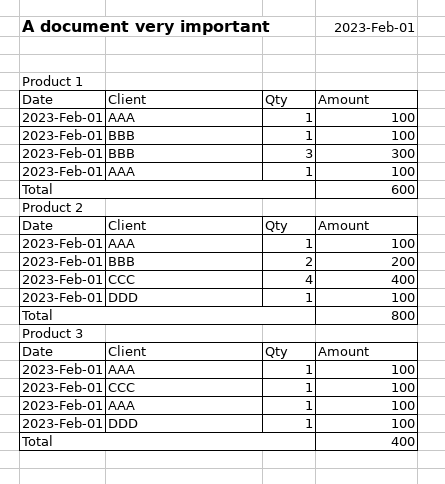
\includegraphics[width=\columnwidth]{spreadsheet_example}
\end{figure}

This document describes a method to classify the different elements of a spreadsheet and build a structure  similar to a JSON file.

\section{Reading Direction}
Cognitive research shows that Human reads a document using a certain direction; depending of the culture and language of
the individual. The human eye is so much trained that it is almost instinctive to look at the top left for any English
reader when a page is displayed on a computer. As such, when a human creates a document, he is influenced by this
reading direction because he supposes his future reader to look at the document in the same way he looks at it. It means
the flow of the various elements of the document will follow the reading direction and therefore can be linked to each
other along this direction.

\subsection{Definition of Reading Direction}
A reading direction is defined by a tuple of a directions. Directions are defined as follows:

\begin{itemize}
    \item Vertical direction when cells are vertically arranged. We can have respectively 2 vertical directions top (T)
    to bottom (B) or bottom (B) to top (T) that we notes respectively TB or BT. 
    \item Horizontal direction when cells are horizontally arranged. We can have respectively 2 horizontal directions
    left (L) to right (R) or right (R) to left (L) that we notes respectively LR or RL. 
    \item The first element of the tuple is the primary direction or line direction and the second element is the
    secondary direction or character direction.
\end{itemize}

Few examples:

\begin{itemize}
    \item TB-LR defines the English direction of reading when we read lines from top to bottom and characters from left
    to right. This direction is sometimes called Gutenberg direction.
    \item TB-RL defines the Arab direction of reading when we read lines from top to bottom and characters from right to
    left
    \item RL-TB defines the traditional Chinese direction of reading when we read lines from right to left and
    characters top to bottom
\end{itemize}

\section{Feature Extraction}
A spreadsheet is composed of unstructured text and of tabular data. Tabular data is a rectangle tightly grouped cells
along rows and columns.

We propose the following steps to extract the free text and the tabular data:

\subsection{Spreadsheet To Bitmap}
Transform the spreadsheet by an bitmap:

\begin{lstlisting}[language=Python, caption=Spreadsheet To Bitmap]
def spearsheet_to_bitmap(rows):
    for row in rows:
      for cell in row:
        if cell.ispace():
          yield 0
        else:
          yield 1
\end{lstlisting}

For example:

\begin{figure}[H]
\caption{Spreadsheet To Bitmap}
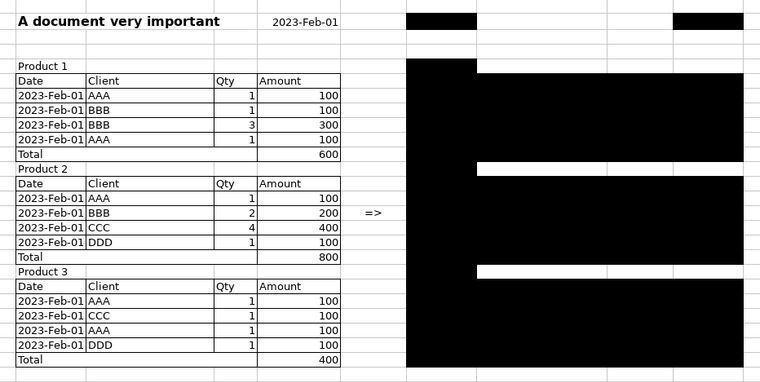
\includegraphics[width=\columnwidth]{spreadhseet_to_bitmap}
\end{figure}

\subsection{Feature Extraction From Bitmap}
From the bitmap, run a feature extraction such as Hough transformation or Region of Interest or even better a package
like OpenCV. In our Java implementation, we use a simple Hough transformation with a convolution (size=3x3, stride=1)
over the bitmap and a kernel (3x3) to detect rectangle corners.

For example:

\begin{figure}[H]
\caption{Feature Extraction}
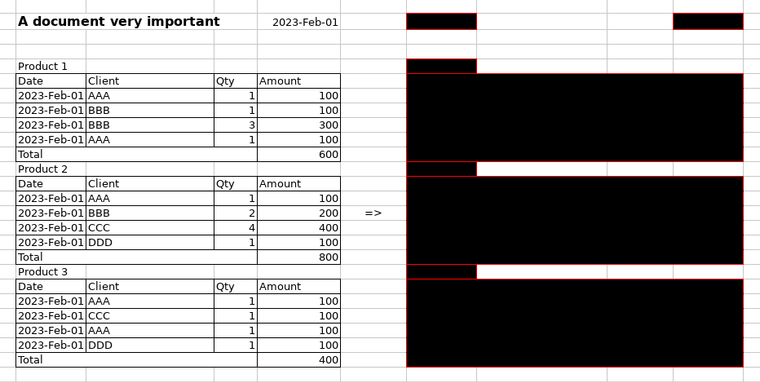
\includegraphics[width=\columnwidth]{feature_extraction}
\end{figure}

\subsection{Classify Features}
Calculate the area of each rectangle and determine if the rectangle enclose unstructured text (here after
called META) or tabular data (here after called TABLE). One easy method is given a threshold, if the area is smaller
than this threshold, the area contains a META else a TABLE:

\begin{lstlisting}[language=Python, caption=Spreadsheet To Bitmap]
def area(r):
  return r.rows * r.cols
  
def classify(RECTANGLES, THRESHOLD):
  for r in RECTANGLES:
    if area(r) < THRESHOLD:
      return "META"
    else:
      return "TABLE"
\end{lstlisting}

For example with a threshold of 1:

\begin{figure}[H]
\caption{Classify Feature}
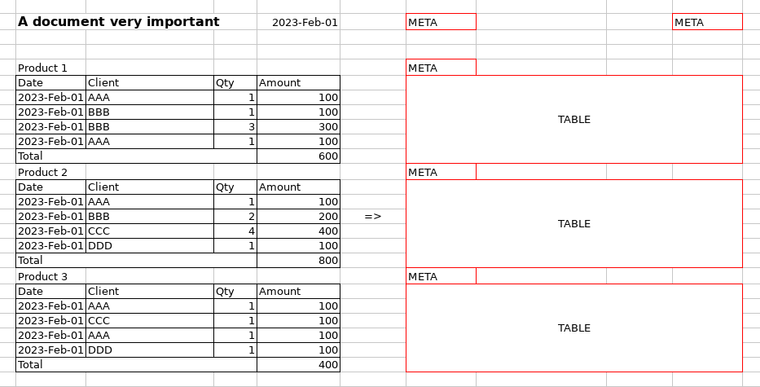
\includegraphics[width=\columnwidth]{classify_features}
\end{figure}

\subsection{Build Tree Structure}
Depending of the reading direction, build a tree linking the META and TABLES found above:

\begin{lstlisting}[language=Python, caption=Tree Structure]
# Define reading direction for english
# document start on the top, left
reading_direction_start_cell = { "row": 0, "col": 0 }

# Child meta are strictly on the right and below a
# current element
reading_direction_next_meta =
        lambda x, y: x.row >= y.row and x.col > y.col

# Child table are on the right and below a current
# element
reading_direction_next_table =
        lambda x, y: x.row >= y.row and x.col >= y.col

def reading_direction_findclosestfromstart():
    closest = None
    min = 0
    for meta in METAS:
        dist = (meta.row - 
                reading_direction_start_cell.row)**2
                + (meta.col -
                reading_direction_start_cell.col)**2
        if closest is None or min < dist:
            closest = meta
            min = dist
        return closest


def reading_direction_ischildof(root, elem, func):
    closest = None
    min = 0
    for node in root:
        if node != elem and func(elem, node):
            dist = (node.row - 0)**2 + (node.row - 0)**2
            if closest is None or min < dist:
            closest = elem
            min = dist
        return closest


root = reading_direction_findclosestfromstart()

# METAS are processed first and serve as anchor
# for the TABLES
for meta in METAS:
    parent = reading_direction_ischildof(
            root,
            meta,
            reading_direction_next_meta
        )
    if parent is None:
    root.append(meta)
    else:
    parent.append(meta)
    
# TABLES are processed in second and possibliy
# attached to METAS
for table in TABLES:
    parent = reading_direction_ischildof(
            root,
            table,
            reading_direction_next_table
        )
    if table is None:
    root.append(table)
    else:
    parent.append(table)
\end{lstlisting}

For example:

\begin{figure}[H]
\caption{Tree Structure}
\includegraphics[width=0.6\columnwidth]{tree_structure.drawio}
\end{figure}

\section{From Tree Structure to JSON structure}
The tree structure above can be easily converted into a JSON structure. Below the final JSON structure of the
spreadsheet:

\begin{lstlisting}[caption=JSON Structure]
[
    {
		"meta": "A document very important",
		"meta": "2023-Feb-01"
    },
    {
		"meta": "Product 1",
		"table": 
		[
            {
                "Date": "2023-Feb-01", 
                "Client": "AAA", "Qty": 1,
                "Amount": 100
            },
        ]
    },
    {
		"meta": "Product 2",
		"table": 
		[
			{
                "Date": "2023-Feb-01",
                "Client": "AAA", "Qty": 1,
                "Amount": 100
            },
        ]
    },
    {
		"meta": "Product 3",
		"table": 
		[
			{
                "Date": "2023-Feb-01",
                "Client": "AAA", "Qty": 1,
                "Amount": 100
            },
        ]
    }
]
\end{lstlisting}

\section{From JSON structure to Tabular Output}
As a complementary to this method, we give the pseudo Python code to transform any JSON structure into Tabular Outputs:

\begin{lstlisting}[language=Python, caption=JSON structure to Tabular Output]
import csv
import json


def is_list_of_list(l):
    return len(l) > 0 and all([
        isinstance(e, list)
        for e in l
    ])


def flatten_list_of_list(l):
    if all([is_list_of_list(e) for e in l]):
        return [
            x for e in l
            for x in flatten_list_of_list(e)
        ]
    else:
        return l


def json_to_tabular_rec(o, column_prefix, rows, headers):
    if isinstance(o, dict):
        for k, v in o.items():
            _, rows = json_to_tabular_rec(
                    v,
                    column_prefix + "." + k,
                    rows,
                    headers
                )
        return headers, rows
    elif isinstance(o, list):
        return headers, flatten_list_of_list(
            [
                json_to_tabular_rec(
                        x,
                        column_prefix,
                        rows,
                        headers
                    )[1]
                for x in o
            ]
        )
    else:
        headers.add(column_prefix)
        if is_list_of_list(rows):
            return headers, [
                    a + [(column_prefix, o)]
                    for a in rows
                ]
        else:
            return headers, rows + [(column_prefix, o)]


def json_to_tabular(o):
    return json_to_tabular_rec(o, "column", [], set())

def tabular_to_csv(headers, rows, fp):
    writer = csv.writer(
            fp,
            delimiter=';',
            quoting=csv.QUOTE_MINIMAL
        )
    writer.writerow(list(headers))
    for row in rows:
        records = [""] * len(headers)
        for cell in row:
            index = list(headers).index(cell[0])
            records[index] = cell[1]
        writer.writerow(records)

with open("example3.json", "r") as fp1:
    with open("example3.csv", 'w', newline='') as fp2:
        tabular_to_csv(
                *json_to_tabular(json.load(fp1)), fp2)
\end{lstlisting}

\section{References}

Han, S., Northoff, G. Reading direction and culture. Nat Rev Neurosci 9, 965 (2008).
\hyperlink{https://doi.org/10.1038/nrn2456-c2}{https://doi.org/10.1038/nrn2456-c2}

\section{Implementation}

Java - \hyperlink{https://github.com/RomualdRousseau/Any2Json}{github}


\end{document}